\documentclass{article}
\usepackage{graphicx} % Required for inserti
\usepackage{caption}
\usepackage{subcaption}
\usepackage{geometry}
\usepackage{blindtext}
\usepackage{amsmath}
\usepackage{amsfonts}
\usepackage{amssymb}
\usepackage{tokcycle}
\usepackage{color}
\usepackage{soul}
\usepackage{xcolor}
\usepackage{wrapfig}
\usepackage{pifont}
\usepackage{xifthen}
\usepackage{multirow}
\usepackage{hyperref}
\usepackage{authblk}
\usepackage[numbers]{natbib}
\usepackage{tikz}
\usepackage{pgfplots}
\usepackage{algorithm}
\usepackage{algpseudocode}
\usepackage{scalerel}
\usetikzlibrary{positioning, decorations.pathreplacing,calligraphy, calc, shapes.geometric, intersections, arrows}
\usepgfplotslibrary{fillbetween}
\pgfplotsset{compat=1.18}


\newcommand{\fmri}{functional magnetic resonance imaging}
\newcommand{\FMRI}{Functional magnetic resonance imaging}
\newcommand{\fmriabbrv}{fMRI}
\newcommand{\eeg}{electroencephalography}
\newcommand{\EEG}{Electroencephalography}
\newcommand{\eegabbrv}{EEG}
\newcommand{\correction}[1]{#1}
\newcommand{\verify}[1]{\textcolor{red}{[VERIFY: #1]}}

%\renewcommand{\hl}[1]{#1}

\setcounter{page}{1}

\date{}
\title{Does EEG to fMRI Synthesis Aid Medical Decision?\\ A Leakage-Audited Evaluation in Psychosis, Schizophrenia and Parkinson's Disease}
\author{}

\newtheorem{proposition}{Proposition}
\newtheorem{theorem}{Theorem}
\newtheorem{lemma}{Lemma}
\newtheorem{corollary}{Corollary}
\newtheorem{proof}{Proof}

\begin{document}

\maketitle

\begin{abstract}
Electroencephalography (EEG) is inexpensive and portable, while functional magnetic resonance imaging (fMRI) provides spatially rich measures of brain function at high cost. EEG-to-fMRI synthesis has been proposed to bring fMRI-like information to EEG-only clinical settings, and synthesized fMRI has been used to classify patients. We test whether it helps. Four EEG-to-fMRI synthesizers (a CNN with topographical attention and random Fourier features, E2fNet, Spec2VolCAMU-Net and NT-ViT) were trained on the NODDI simultaneous EEG-fMRI dataset with a corrected, scanner-trigger-aligned protocol and applied to resting EEG from five public cohorts: two first-episode psychosis samples ($n=77$, $n=61$), chronic schizophrenia ($n=77$), Parkinson's disease ($n=50$) and a task-EEG schizophrenia-spectrum sample ($n=43$). Each cohort was classified from EEG band power, synthesized fMRI and their combination with linear classifiers under repeated cross-validation and permutation tests, with untrained (random-weight) synthesizers as an architecture-only control; the contrastive sinusoid-separation method of our earlier work was re-evaluated alongside. A leakage audit preceded the benchmark: in the task-EEG cohort, the auxiliary-channel layout differs between patients and controls, and our earlier synthesized-fMRI pipeline (stft view AUC $0.93$) drops to chance ($0.49$) once those channels are removed. Band power separated Parkinson's disease from controls (AUC $0.79$) but not the psychosis or schizophrenia cohorts (AUC $0.54$--$0.65$). Synthesized fMRI classified Parkinson's disease (best AUC $0.74$) but never outperformed band power, untrained synthesizers matched it (AUC $0.70$--$0.74$), and contrastive fine-tuning reached at most AUC $0.70$. On NODDI, the synthesizers did not beat an EEG-free template, and EEG explained a negligible part of preprocessed BOLD (parcel $r\approx0.03$, $R^2\approx0$). In these cohorts, synthesized fMRI carries EEG spectral information rather than learned haemodynamics, and does not improve EEG-based diagnosis.
\end{abstract}

\section{Introduction}\label{section:introduction}

fMRI resolves brain activity in space but is costly and scarce, especially in low-resource settings \cite{ogbole2018survey}; EEG is cheap and portable but spatially coarse. EEG-to-fMRI synthesis learns, from simultaneous recordings, a mapping from scalp EEG to BOLD volumes, and has been proposed as a way to obtain fMRI-like information where only EEG is available \cite{liu2019convolutional, liu2020latent, bricman2021eeg2fmri, calhas2022eeg, roos2025brainwaves, he2025spec2vol, lanzino2024ntvit, li2024neurobolt}. Schizophrenia and related psychotic disorders are a natural target: they are clinically heterogeneous \cite{saha2005systematic}, their diagnosis draws on psychological, neuroimaging, molecular and speech-based assessments \cite{andreou2020structural,neale2015genetic,corcoran2020language}, and both EEG \cite{tan2016eeg,aydin2018cortical,roach2008event,bates2009low} and fMRI \cite{oh2020identifying, velakoulis2006hippocampal, haukvik2013schizophrenia} carry group differences. Parkinson's disease, with well-documented resting EEG alterations, offers a second target. Two studies have classified patients from synthesized fMRI: schizophrenia from a task-EEG cohort, in an earlier version of this work \cite{calhas2023medrxiv}, and Parkinson's disease from eight subjects of a resting-EEG cohort \cite{yao2025catd}.

Whether synthesized fMRI adds diagnostic information beyond the EEG it is computed from has not been tested with the controls such a claim requires: classification data free of shortcuts unrelated to the disease; a comparison, under identical validation, with an EEG-only view and with the combination of both; and a test of whether any discrimination comes from the learned EEG-to-fMRI mapping or from the network architecture alone, which can be done by applying the same networks with untrained weights. We report such an evaluation. We also re-examine our earlier result, which did not survive it.

\textbf{Key contributions:} (1) a leakage audit of public clinical EEG cohorts, showing that our earlier schizophrenia result is explained by a group-dependent auxiliary-channel layout; (2) a classification benchmark of four EEG-to-fMRI synthesizers and of the contrastive sinusoid-separation method \cite{calhas2023medrxiv} on five public cohorts covering first-episode psychosis, chronic schizophrenia, a schizophrenia-spectrum task cohort and Parkinson's disease, with EEG-only, fusion, untrained-network and permutation controls; (3) supporting evidence on what the synthesizers learn: a scanner-trigger-aligned training protocol for the NODDI dataset, an EEG-free template baseline, and a fair-target test of how much BOLD variance EEG predicts.

\subsection*{Problem description}\label{section:problem_description}

Let $\mathcal{V} = \{v_1, \dots, v_n\}$ be a set of different views, such that $\forall i \in \{1, \dots, n\}: v_i = \{F_i, \theta_i\}$. A view $v_i$ is characterized by a function structure, $F_i$, and its parameters, $\theta_i$. Each projection $F_i: \mathbb{R}^{D_0} \to \mathbb{R}^{D_i}$ is performed from the original feature space, $\mathbb{R}^{D_0}$, to its view space, $\mathbb{R}^{D_i}$. Each subject's recording, $\vec{x}_0$, is paired with a label $y \in \{0,1\}^K: \sum_k y_k=1$, where $K=2$ (patient or control). A view, $v_i$, is evaluated by a linear classifier minimizing
\begin{equation}\label{equation:loss}
    \mathcal{L}_C(\vec{x}_0, y) = -y \times \mbox{log}(\sigma(W^i_f \cdot  v_i(\vec{x}_0) + b^i_f)),
\end{equation}
where $W^i_f \in \mathbb{R}^{K \times D_i}$ and $b^i_f \in \mathbb{R}^K$ are the parameters of the linear classifier, referred to as $\theta_C^i = W^i_f \bigcup b^i_f$, using the softmax activation, $\sigma$, plus an $l_2$ penalty on $W^i_f$. The question is whether a synthesized \textit{fmri} view, alone or added to an EEG view, lowers the expected loss on unseen subjects relative to the EEG view alone.

\section{Background: Defining the EEG views}\label{section:eeg_views}

This section defines the views compared in our experiments: an EEG spectral view, \textit{bandpower}; the time-frequency representation that feeds the synthesizers, \textit{stft}; and the synthesized fMRI, \textit{fmri}, produced by four synthesizers. The earlier version of this work also used a \textit{raw} channel-temporal view; in that implementation the EEG was resampled to one sample every two seconds before classification, which removes almost all EEG content, and its below-chance AUC ($0.225$) is the behaviour of a feature set without signal under leave-one-subject-out validation \cite{varoquaux2018}. We do not use it.

\subsection{\textit{bandpower} view}\label{eeg_views:bandpower}

Frequency-domain EEG features are long-established markers in schizophrenia and Parkinson's disease \cite{itil1977qualitative,roach2008event,bates2009low,barros2021advanced}. We use the simplest such view: for each of the $C=57$ channels (Section~\ref{section:adaptation}), Welch power spectra (4\,s windows) summarised as relative log power in five bands (1--4, 4--8, 8--13, 13--30, 30--45\,Hz), so $v_0(\vec{x}_0) \in \mathbb{R}^{C\times5}$. Band power is spatially organised over the scalp and clinically interpretable, so it is both the natural EEG-only baseline and the information any synthesized view starts from.

\subsection{\textit{stft} view}\label{eeg_views:channel_freq_time}

Research studies, along the years, have had a common trend of extracting time frequency features from the EEG signal \cite{fingelkurts2007impaired,burgess2002functional,albrecht2018time,roach2008event,bates2009low}. The synthesizers take a short-time Fourier representation \cite{jacobsen2003sliding} as input, $v_1=\{F_1, \theta_1\}$ with $\vec{x}_1 \in \mathbb{R}^{D_1}$, $D_1 = C \times F \times T$: log-magnitude spectra of $T=20$ consecutive EEG segments of one fMRI repetition time (TR, 2.16\,s) each, between 0.46 and 45\,Hz ($F=97$ bins), i.e. the 43.2\,s of EEG preceding an fMRI volume, which covers the haemodynamic delay. This view is not classified directly; it defines the input of the \textit{fmri} views.

\subsection{EEG to fMRI synthesis: \textit{fmri} view}\label{eeg_views:eeg_to_fmri}


\begin{figure*}[!t]
    \centering
    \begin{tikzpicture}
        [inner sep=2mm, scale=0.87]

        \node (x) at (0,0) {};
        
        \node (stft) at ($(x)+(-1.2,0.3)$) {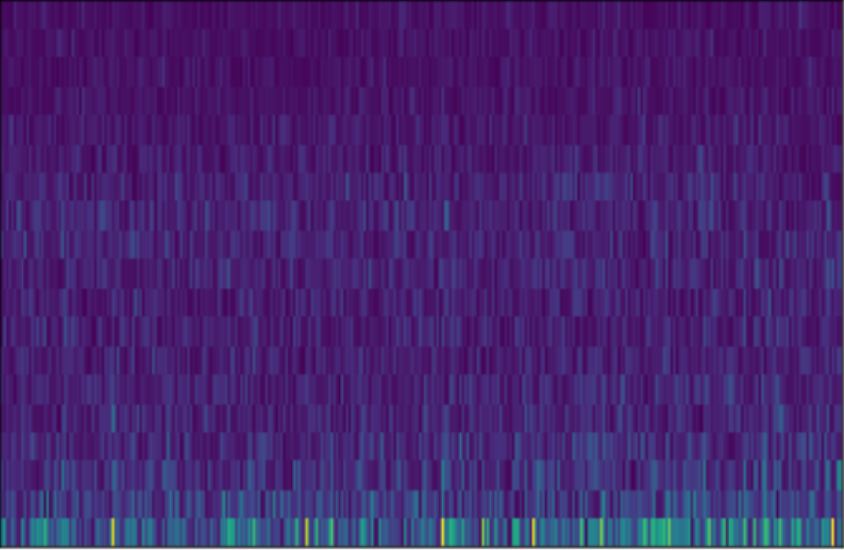
\includegraphics[width=0.1\textwidth]{stft.png}};
        \node (stft) at ($(stft)+(0.1,-0.1)$) {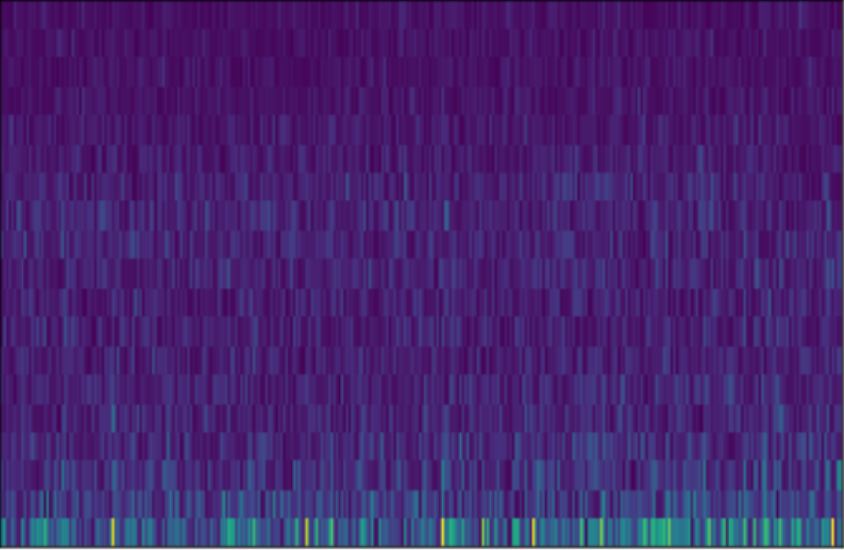
\includegraphics[width=0.1\textwidth]{stft.png}};
        \node (stft) at ($(stft)+(0.1,-0.1)$) {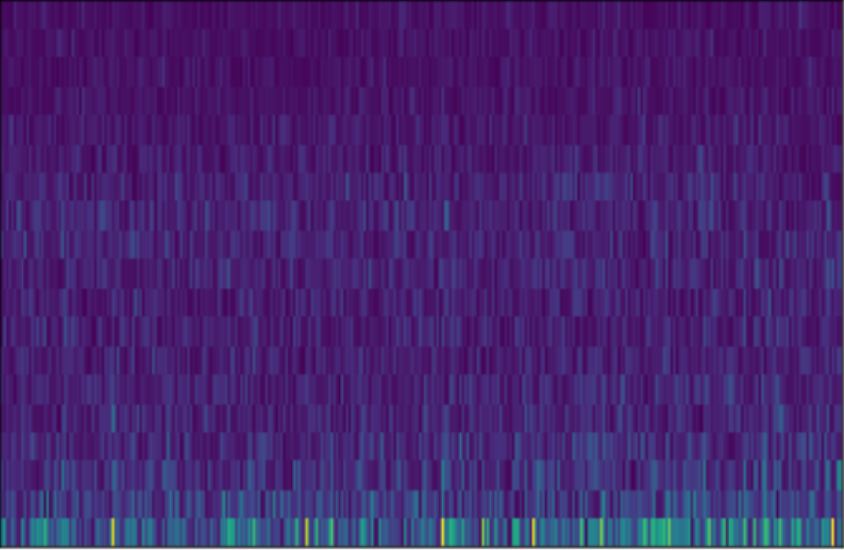
\includegraphics[width=0.1\textwidth]{stft.png}};
        \node (stft) at ($(stft)+(0.1,-0.1)$) {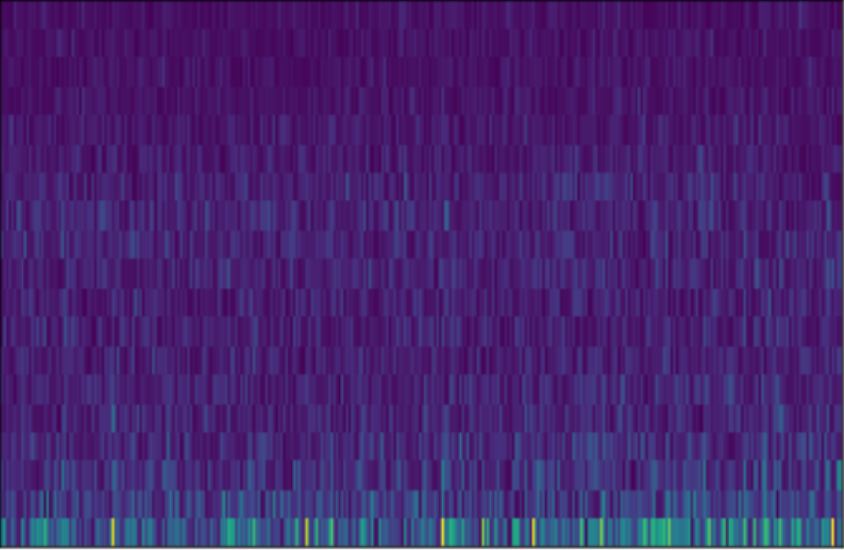
\includegraphics[width=0.1\textwidth]{stft.png}};
        \node (stft) at ($(stft)+(0.1,-0.1)$) {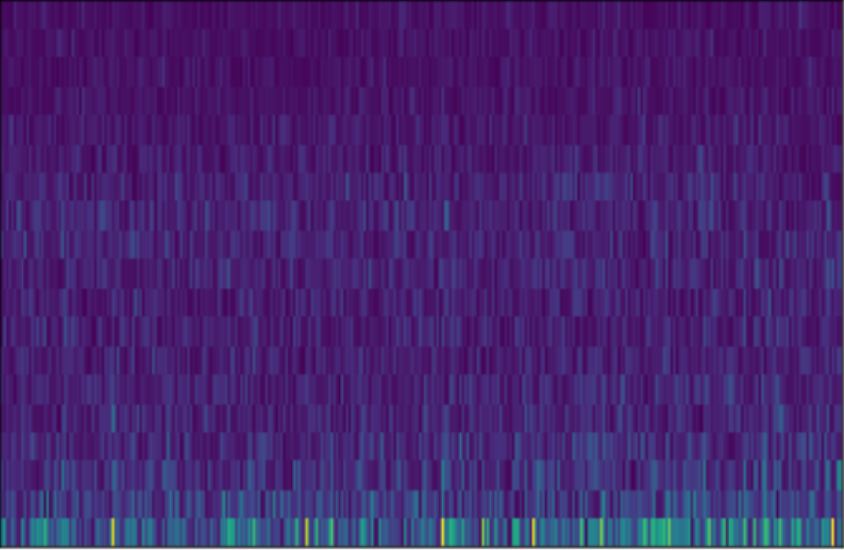
\includegraphics[width=0.1\textwidth]{stft.png}};
        
        \node at ($(stft)+(-0.2,-0.9)$) {$\vec{x}_1$};
        
        \node (encoder) at ($(x)+(2.3,0)$) {\tikz {\draw[rounded corners, draw=black!50,fill=black!20,thick, dash pattern=on 7pt off 2pt] (0,0) rectangle ++(3.4,3);}};
        \node (decoder) at ($(x)+(7.8,0)$) {\tikz {\draw[rounded corners, draw=brown!70,fill=green!20,thick, dash pattern=on 7pt off 2pt] (0,0) rectangle ++(4.5,3);}};
        \node (legend_encoder) at ($(encoder)+(0,-1.9)$) {Encoder};
        \node (legend_decoder) at ($(decoder)+(0,-1.9)$) {Decoder};
        
        
        \node (channel_organization) at ($(x)+(1,0)$) {\tikz {\draw[draw=blue!50,fill=blue!20,thick] (0,0) rectangle ++(0.3,2);}};

        \node (T) at ($(channel_organization)+(0.7,0)$) {$T$};

        \node (resblock1) at ($(T)+(0.7,0)$) {\tikz {\draw[rounded corners, draw=red!40,fill=red!20,thick] (0,0) rectangle ++(0.3,2);}};

        \node (resblock2) at ($(resblock1)+(0.7,0)$) {\tikz {\draw[rounded corners, draw=red!40,fill=red!20,thick] (0,0) rectangle ++(0.3,2);}};

        \node (latent_affine) at ($(resblock2)+(0.7,0)$) {\tikz {\draw[draw=orange!40,fill=orange!20,thick] (0,0) rectangle ++(0.3,2);}};

        \node (latent) at ($(latent_affine)+(1,0)$) {$\vec{z}$};

        \node (fourier) at ($(latent)+(2,0)$) {$cos(\omega \cdot \vec{z} + \beta)$};

        \node (style) at ($(fourier)+(2,0)$) {$\odot $};
        \node (style_weight) at ($(style)+(0,1.3)$) {$W$};

        \node (decoder_affine) at ($(style)+(1,0)$) {\tikz {\draw[draw=orange!40,fill=orange!20,thick] (0,0) rectangle ++(0.3,2);}};

        \node (output) at ($(decoder_affine)+(1.7,0)$) {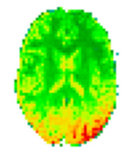
\includegraphics[width=0.1\textwidth]{fmri.png}};
        \node at ($(output)+(0,-1.3)$) {$\vec{x}_2$};
        
        
        \draw[-latex, line width=1pt, black!60] ($(x)+(0.2,0)$) -- ($(channel_organization)+(-0.25,0)$);
        \draw[-latex, line width=1pt, black!60] ($(channel_organization)+(0.2,0)$) -- ($(T)+(-0.2,0)$);
        \draw[-latex, line width=1pt, black!60] ($(T)+(0.2,0)$) -- ($(resblock1)+(-0.2,0)$);
        \draw[-latex, line width=1pt, black!60] ($(resblock1)+(0.2,0)$) -- ($(resblock2)+(-0.2,0)$);
        \draw[-latex, line width=1pt, black!60] ($(resblock2)+(0.2,0)$) -- ($(latent_affine)+(-0.2,0)$);
        \draw[-latex, line width=1pt, black!60] ($(latent_affine)+(0.25,0)$) -- ($(latent)+(-0.25,0)$);
        \draw[-latex, line width=1pt, black!60] ($(latent)+(0.25,0)$) -- ($(fourier)+(-1.25,0)$);
        \draw[-latex, line width=1pt, black!60] ($(fourier)+(1.25,0)$) -- ($(style)+(-0.25,0)$);
        \draw[-latex, line width=1pt, black!60] ($(style)+(0.25,0)$) -- ($(decoder_affine)+(-0.25,0)$);
        \draw[-latex, line width=1pt, black!60] ($(decoder_affine)+(0.25,0)$) -- ($(output)+(-0.8,0)$);
        \draw[-latex, line width=2pt, red!60] ($(style_weight)+(0,-0.25)$) -- ($(style)+(0,0.25)$);
        
        \node (attention_legend) at ($(encoder)+(-3.5,-3.4)$) {\tikz {\draw[draw=blue!50,fill=blue!20,thick] (0,0) rectangle ++(0.3,2);}};
        \node (resblock_legend) at ($(attention_legend)+(2.5,0)$) {\tikz {\draw[rounded corners, draw=red!40,fill=red!20,thick] (0,0) rectangle ++(0.3,2);}};
        \node (affine_legend) at ($(resblock_legend)+(3,0)$) {\tikz {\draw[draw=orange!40,fill=orange!20,thick] (0,0) rectangle ++(0.3,2);}};
        \node (hadamard_legend) at ($(affine_legend)+(3.8,0)$) {$\odot$};

        \node[align=left] at ($(affine_legend)+(1.7,0)$) {Affine projection};
        \node[align=left] at ($(attention_legend)+(1.1,0)$) {Attention};
        \node[align=left] at ($(resblock_legend)+(1.4,0)$) {Resnet block};
        \node at ($(hadamard_legend)+(2.,0)$) {Hadamard product};
        
    \end{tikzpicture}
    \caption{The neural architecture has two components: an Encoder (shaded in grey) and a Decoder (shaded in green). The input is the \textit{stft} $v_1$ representation. The output is the synthesized \textit{fmri}. The Encoder begins with a simple attention mechanism on the channels dimension of the \textit{stft}. After, it is processed by two Resnet blocks and an affine layer. This produces the latent representation $\vec{z}$. Following, the Decoder picks this representation and builds the cosine bases through the projection $\omega \cdot \vec{z} + \beta$. The sinusoids are style induced with $cos(\omega \cdot \vec{z} + \beta)\odot W$. The vector $W$ is a style fixed pretrained vector of an \textit{fmri} representation, learned from a simultaneous EEG and fMRI dataset (described in Section \ref{section:fmri_data}). Finally, an affine layer projects it to the \textit{fmri} space.}
    \label{fig:horizontal_architecture}
\end{figure*}


The first synthesizer is the network introduced and validated in our earlier work \cite{calhas2022eeg}; its architecture is adopted from that study, not proposed here, and the present work re-implements it in PyTorch and retrains it with the protocol of Section~\ref{section:fmri_data}. We refer to it as CNN-TAG. Its flow is illustrated in Figure \ref{fig:horizontal_architecture}. Its input is the \textit{stft} view, $\vec{x}_1$; its output is the \textit{fmri} view, $\vec{x}_2 \in \mathbb{R}^{M_1 \times M_2 \times M_3}$, a volume of $64\times64\times30$ voxels. Zooming out of the neural network, we describe this view as $v_2 = \{ F_2, \theta_2\}$, where $F_2 = F_1 \bigcup F$ is the union of the \textit{stft} transform and the network $F$, and $\theta_2 = \theta_1 \bigcup \theta_F$.

In terms of structure, the network processes the input with an attention mechanism over channels. An attention weight matrix $A \in \mathbb{R}^{C \times (F T)}$ is used to compute $E \in \mathbb{R}^{C \times C}$, $E_{ij} = \vec{x}_i^\top A_j$, which is normalised with sparsemax along $j$ to give $B$; the attention-processed representation is
\begin{equation}\label{equation:attention_output}
    T_i  = \sum_j^C b_{ij}\, \vec{x}_j, \forall i \in \{1, \dots, C\}.
\end{equation}
$T$ is processed by two residual blocks \cite{he2016deep} and a fully connected layer, whose parameters $\theta_E$ form the encoder. The encoder output projects random Fourier features \cite{rahimi2007random,tancik2020fourier}, parameterized by $\omega$ and $\beta$ and layer-normalised around $\pi/2$; the resulting sinusoids are multiplied with a learned latent style vector, $W \in \mathbb{R}^L$, and an affine transformation maps them to the fMRI volume space. With this, we formulate the function structure $F: \mathbb{R}^{C \times F \times T} \to \mathbb{R}^{D_2}$.

\noindent\textbf{Other synthesizers.} Three published synthesizers were trained with the same data and protocol, using the authors' model code: \textbf{E2fNet} \cite{roos2025brainwaves}, a convolutional EEG encoder followed by a 2D U-Net and a convolutional fMRI decoder; \textbf{Spec2VolCAMU-Net} \cite{he2025spec2vol}, a multi-scale convolutional spectrogram encoder with temporal self-attention and a Vision-Mamba U-Net decoder, whose selective scan we computed with an exact pure-PyTorch chunked recurrence because the CUDA kernel was unavailable; and \textbf{NT-ViT} \cite{lanzino2024ntvit}, a mel-spectrogram vision-transformer encoder and decoder with a domain-matching loss, which computes its own spectrograms and therefore received the same 43.2\,s window as raw waveforms (the published model used a simultaneous 2.16\,s window without haemodynamic lag). CATD \cite{yao2025catd} could not be included because no code is available; NeuroBOLT and UnEBOLT \cite{li2024neurobolt,li2026unebolt} predict parcel time series rather than volumes and were used in the supporting fidelity analyses only.

\noindent\textbf{Untrained controls.} For each synthesizer, the same architecture with random initial weights was passed through the identical pipeline. A fixed nonlinear projection of EEG spectra into a voxel grid can support classification on its own; this control separates that effect from the learned EEG-to-fMRI mapping.

\section{Adaptation to new data}\label{section:adaptation}

EEG datasets differ in electrode count and layout, sampling rate, reference and paradigm, which changes their representation in $\mathbb{R}^{C \times T}$. The earlier version of this work adapted the network to each dataset by mutating convolution strides and zero-filling high frequencies. We replace this with a single harmonisation applied to every recording, clinical or not, so that each synthesizer receives inputs in exactly the montage and sampling rate it was trained on:

\noindent\textbf{Channel selection by type.} EEG channels are selected by their declared type, never by position; EOG, ECG, EMG, accelerometer, trigger and auxiliary (EXG) channels are removed. Positional selection is what allowed the label leak described in Section~\ref{section:res_leak}.

\noindent\textbf{Montage harmonisation.} Channels are mapped to standard 10-05 positions and interpolated with spherical splines onto the 57 EEG channels recorded in every NODDI subject (Section~\ref{section:fmri_data}).

\noindent\textbf{Common filtering and resampling.} Notch filtering at the mains frequency and harmonics, 0.5--45\,Hz band-pass, average reference and resampling to 250\,Hz. Frequencies above 45\,Hz are discarded for every dataset, so all synthesizers see the same frequency range.

Clinical EEG has no fMRI volume markers; the synthesizers are applied to consecutive pseudo-TRs of 2.16\,s starting 43.2\,s into each recording, so that every synthesized volume has a full 20-segment history.

\section{Methods}\label{section:methods}

\subsection{EEG Preprocessing and Analysis}

All recordings went through the harmonisation of Section~\ref{section:adaptation} (MNE-Python). Each clinical recording was cropped to a fixed duration per cohort (Table~\ref{tab:data_description}), identical for patients and controls, to remove duration differences between groups. The cleaned NODDI EEG released by the dataset authors, in which scanner (gradient) and pulse (ballistocardiographic) artefacts were removed \cite{dataset_01}, was used as is before harmonisation.

\subsection{fMRI Data Collection and Analysis}\label{section:fmri_data}

fMRI is available only in the synthesis training dataset, NODDI \cite{dataset_01,deligianni2016}; the clinical cohorts are EEG-only and contain no fMRI. In NODDI, fMRI was acquired simultaneously with EEG at rest (eyes open, fixation) on a 1.5\,T Siemens Avanto: T2*-weighted gradient-echo EPI, TR/TE 2160/30\,ms, 30 slices of 3\,mm (1\,mm gap), effective voxel size $3.3\times3.3\times4.0$\,mm, $64\times64\times30$ voxels, 300 volumes; EEG with a 64-channel MR-compatible cap (BrainCap MR), recorded at 5\,kHz, released at 250\,Hz after artefact correction.

Two properties of this release matter for synthesis and, to our knowledge, have not been reported. First, in 15 of the 16 subjects the EEG begins 13--130\,s before the first fMRI volume; pipelines that pair EEG and fMRI from the start of the file, including the one used in the earlier version of this work, pair EEG with volumes 6--60 TRs away. We pair them through the scanner volume markers in the EEG file (one per TR). Second, two electrode montages are present: 10 subjects have F1/F2/C1/C2/P1/P2 and 6 have P9/P10/PO9/PO10/O9/O10, in a different channel order, so positional channel indexing mixes electrodes across subjects. We use the 57 channels recorded in all subjects, selected by name; the ECG channel is excluded.

\noindent\textbf{Synthesizer training.} The synthesis target is the raw EPI volume min--max scaled to $[0,1]$ per volume, the convention of the published volumetric synthesizers. Synthesizers used for classification were trained on 14 NODDI subjects, with two subjects held out to select the training epoch; loss $0.5(1-\mathrm{SSIM})+0.5\,\mathrm{MSE}$, Adam, learning rate $10^{-3}$, batch size 32, mini-batches shuffled across subjects, 50 epochs (15 for Spec2VolCAMU-Net). NT-ViT used the authors' recipe (AdamW, learning rate $5\times10^{-4}$, 30 epochs) with batch size 32 instead of 128, because the 43.2\,s input did not fit in memory at 128. Input features were standardised with training-subject statistics only. NODDI carries no diagnostic labels and is never used for classification.

\noindent\textbf{From synthesized volumes to a subject view.} For each clinical subject, the synthesized volumes (one per pseudo-TR, clipped to $[0,1]$) are summarised by their voxelwise temporal mean and standard deviation, giving $2\times64\times64\times30$ features; this is the \textit{fmri} view classified in Section~\ref{section:setting}.

\subsection{Integration Approach}\label{section:integration}

To fairly compare views, we employ a linear classifier, which allows a direct assessment of representational discriminative power and easy interpretation \cite{treviso2020explanation}. In addition, we re-evaluate the integration approach of the earlier version of this work, which adapts the CNN-TAG synthesizer to the diagnostic task by separating classes in its sinusoid space while the voxel decoder is kept fixed.

For the synthesized fMRI view $v_2$, which involves sinusoidal projections, a challenge arises: separation of data via $y|\vec{x}_1$ may be disrupted. Since EEG data inherently contains label-relevant information, preserving the distribution through the sinusoidal transformation is crucial. We address this by ensuring the projection $y|\omega \cdot \vec{z} + \beta$ maintains the same distribution as $y|\vec{x}_2$, enabling effective class separation while preserving sinusoidal structure.

\subsubsection{Sinusoid separation}\label{methods:separation}

\begin{figure}[ht]
    \centering
    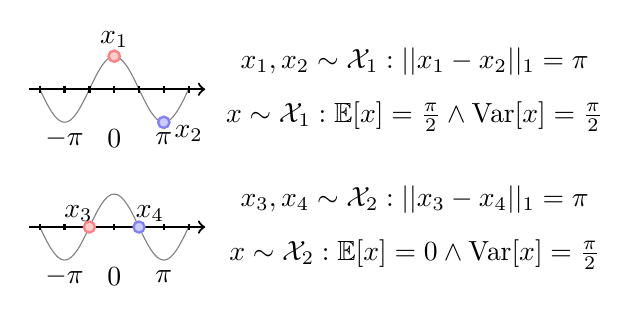
\begin{tikzpicture}
        [scale=0.7,
        inner sep=0.5mm,
        pd/.style={circle,draw=red!50,fill=red!20,thick},
        hc/.style={circle,draw=blue!50,fill=blue!20,thick}]
        
        \node (sinusoid1) at (0,0) {};
        
        \draw[black, thick, ->] ($(sinusoid1)+(-2,0.3)$) -- ($(sinusoid1)+(1.2,0.3)$);%xaxis
        \draw[thin, black!50] ($(sinusoid1)+(0.9,0.3)$) sin ($(sinusoid1)+(0.45,-0.3)$);
        \draw[thin, black!50] ($(sinusoid1)+(0.45,-0.3)$) cos ($(sinusoid1)+(0.,0.3)$);
        \draw[thin, black!50] ($(sinusoid1)+(0.,0.3)$) sin ($(sinusoid1)+(-0.45,0.9)$);
        \draw[thin, black!50] ($(sinusoid1)+(-0.45,0.9)$) cos ($(sinusoid1)+(-0.9,0.3)$);
        \draw[thin, black!50] ($(sinusoid1)+(-0.9,0.3)$) sin ($(sinusoid1)+(-1.35,-0.3)$);
        \draw[thin, black!50] ($(sinusoid1)+(-1.35,-0.3)$) cos ($(sinusoid1)+(-1.8,0.3)$);
        
        
        \draw[black, thick] ($(sinusoid1)+(-1.8,0.36)$) -- ($(sinusoid1)+(-1.8,0.24)$);
        \draw[black, thick] ($(sinusoid1)+(-1.35,0.36)$) -- ($(sinusoid1)+(-1.35,0.24)$);
        \draw[black, thick] ($(sinusoid1)+(-0.9,0.36)$) -- ($(sinusoid1)+(-0.9,0.24)$);
        \draw[black, thick] ($(sinusoid1)+(-0.45,0.36)$) -- ($(sinusoid1)+(-0.45,0.24)$);
        \draw[black, thick] ($(sinusoid1)+(0.,0.36)$) -- ($(sinusoid1)+(0.,0.24)$);
        \draw[black, thick] ($(sinusoid1)+(0.45,0.36)$) -- ($(sinusoid1)+(0.45,0.24)$);
        \draw[black, thick] ($(sinusoid1)+(0.9,0.36)$) -- ($(sinusoid1)+(0.9,0.24)$);
        
        \node at ($(sinusoid1)+(-1.35,-0.6)$) {$-\pi$};
        \node at ($(sinusoid1)+(-0.45,-0.6)$) {$0$};
        \node at ($(sinusoid1)+(0.45,-0.6)$) {$\pi$};
        
        \node (ind1) at ($(sinusoid1)+(-0.45,0.9)$) [pd] {};
        \node (ind1) at ($(sinusoid1)+(0.45,-0.3)$) [hc] {};
        
        \node (ind1) at ($(sinusoid1)+(-0.45,0.9)$) [pd] {};
        \node (ind1) at ($(sinusoid1)+(0.45,-0.3)$) [hc] {};
        
        
        \node (sinusoid2) at ($(sinusoid1)+(0,-2.5)$) {};
        
        \draw[black, thick, ->] ($(sinusoid2)+(-2,0.3)$) -- ($(sinusoid2)+(1.2,0.3)$);%xaxis
        \draw[thin, black!50] ($(sinusoid2)+(0.9,0.3)$) sin ($(sinusoid2)+(0.45,-0.3)$);
        \draw[thin, black!50] ($(sinusoid2)+(0.45,-0.3)$) cos ($(sinusoid2)+(0.,0.3)$);
        \draw[thin, black!50] ($(sinusoid2)+(0.,0.3)$) sin ($(sinusoid2)+(-0.45,0.9)$);
        \draw[thin, black!50] ($(sinusoid2)+(-0.45,0.9)$) cos ($(sinusoid2)+(-0.9,0.3)$);
        \draw[thin, black!50] ($(sinusoid2)+(-0.9,0.3)$) sin ($(sinusoid2)+(-1.35,-0.3)$);
        \draw[thin, black!50] ($(sinusoid2)+(-1.35,-0.3)$) cos ($(sinusoid2)+(-1.8,0.3)$);
        
        
        \draw[black, thick] ($(sinusoid2)+(-1.8,0.36)$) -- ($(sinusoid2)+(-1.8,0.24)$);
        \draw[black, thick] ($(sinusoid2)+(-1.35,0.36)$) -- ($(sinusoid2)+(-1.35,0.24)$);
        \draw[black, thick] ($(sinusoid2)+(-0.9,0.36)$) -- ($(sinusoid2)+(-0.9,0.24)$);
        \draw[black, thick] ($(sinusoid2)+(-0.45,0.36)$) -- ($(sinusoid2)+(-0.45,0.24)$);
        \draw[black, thick] ($(sinusoid2)+(0.,0.36)$) -- ($(sinusoid2)+(0.,0.24)$);
        \draw[black, thick] ($(sinusoid2)+(0.45,0.36)$) -- ($(sinusoid2)+(0.45,0.24)$);
        \draw[black, thick] ($(sinusoid2)+(0.9,0.36)$) -- ($(sinusoid2)+(0.9,0.24)$);
        
        \node at ($(sinusoid2)+(-1.35,-0.6)$) {$-\pi$};
        \node at ($(sinusoid2)+(-0.45,-0.6)$) {$0$};
        \node at ($(sinusoid2)+(0.45,-0.6)$) {$\pi$};
        
        \node (ind1) at ($(sinusoid2)+(-0.9,0.3)$) [pd] {};
        \node (ind1) at ($(sinusoid2)+(0.,0.3)$) [hc] {};
        
        
        \node at ($(sinusoid1)+(-0.45,1.2)$) {$x_1$};
        \node at ($(sinusoid1)+(0.9,-0.5)$) {$x_2$};
        
        \node at ($(sinusoid2)+(-1.1,0.55)$) {$x_3$};
        \node at ($(sinusoid2)+(0.2,0.55)$) {$x_4$};
        
        \node (distance1) at ($(sinusoid1)+(5,0.8)$) {$x_1, x_2 \sim \mathcal{X}_1: ||x_1-x_2||_1=\pi$};
        \node at ($(distance1)+(0,-1)$) {$x \sim \mathcal{X}_1: \mathbb{E}[x] = \frac{\pi}{2} \wedge \mbox{Var}[x]=\frac{\pi}{2}$};
        
        \node (distance2) at ($(sinusoid2)+(5,0.8)$) {$x_3, x_4 \sim \mathcal{X}_2: ||x_3-x_4||_1=\pi$};
        \node at ($(distance2)+(0,-1)$) {$x \sim \mathcal{X}_2: \mathbb{E}[x] = 0 \wedge \mbox{Var}[x]=\frac{\pi}{2}$};
    \end{tikzpicture}
    \caption{Description of how two similarly distributed samples, taken from $\mathcal{X}_1$ and $\mathcal{X}_2$, can lead to different portions of the cosine function image, since a sinusoid is periodic. Two distributions $\mathcal{X}_1$ and $\mathcal{X}_2$, may be mapped to the same image (second/bottom example). This is why a cosine is a shift invariant function. However, there are intervals a shift can be made and it is not invariant. Such intervals take the form $\forall i \in \mathbb{Z}: [i \pi, (i+1)\pi]$.}
    \label{fig:normalization_shift}
\end{figure}

In order to separate data along the projection of cosines, we have to operate in a sub-domain interval where the $cos$ is not periodic. Layer normalization \cite{ba2016layer}, with center in $\frac{\pi}{2}$ and standard deviation of $\frac{\pi}{2}$, maps most of the data to such an interval of the cosine. See Figure \ref{fig:normalization_shift} for an illustration example.

Nonetheless, the assurance that the projections are likely in a non periodic sub-domain of the cosine function, does not alone complete separation of the data. This is because the distribution $y|\omega \cdot \vec{z} +\beta$ needs to be separated accordingly. We propose a modified contrastive loss defined as
\begin{equation}\label{equation:contrastive}
    \mathcal{L}_D(p_1, p_2, y_p) = y_p \times D(p_1, p_2) + (1-y_p) \times ||D(p_1,p_2)-m||_1,
\end{equation}
where $p_1, p_2$ formulate a pair of two instances and $y_p \in \{0,1\}$ defines the pairwise label, being $0$ when the label of $p_1, p_2$ mismatch and $1$ when they match. $D(p_1,p_2)$ is the $l$1 distance $||p_1-p_2||_1^1$. Setting $m\in[\epsilon, \pi]: \epsilon>0$, together with the described layer normalization, allows separation of the data within a non periodic sub domain of the cosine. The minimization of $\mathcal{L}_D$, together with the layer normalization, separates the data when projected by the cosine function, as formalised below (proof in the Appendix).
\begin{theorem}[Separation under Cosine Projection]
Let $z_1, z_2 \in \mathbb{R}^d$ be two latent vectors such that each coordinate lies in $[0, \pi]$. Let the projection be defined as
\[
\phi(z) = \cos(\omega^\top z + \beta),
\]
where $\omega \sim \mathcal{N}(0, I_d)$ and $\beta \sim \mathrm{Uniform}[0, 2\pi]$. Then, for $\|z_1 - z_2\|_2 \geq \epsilon > 0$, the expected cosine similarity between $\phi(z_1)$ and $\phi(z_2)$ satisfies
\[
\mathbb{E}_{\omega, \beta}[\phi(z_1)^\top \phi(z_2)] < d.
\]
Moreover, this expected similarity decreases exponentially with increasing $\|z_1 - z_2\|_2$, so a contrastive margin $m$ that increases the latent distance between classes decreases their expected similarity after projection.
\end{theorem}
In Figure \ref{fig:sinusoid_separation}, we illustrate the effects of this methodology, before and after the learning session.

\noindent\textbf{Training.} The encoder is trained with $\mathcal{L}_D$ on pairs of EEG windows, while a linear classifier with an $l_1$ penalty is trained with $\mathcal{L}_C$ on the synthesized volume (detached from the encoder); the style vector and the voxel decoder stay frozen at their NODDI weights. Each synthesized window is an instance, and a subject's score is the mean predicted probability over its windows. We run two variants: \emph{as in 2023}, in which the encoder and Fourier projection are re-initialised (what the earlier implementation did, so that its synthesized fMRI never used the learned mapping), and \emph{pretrained}, in which they start from the NODDI-trained synthesizer and are fine-tuned. Training uses a fixed budget (10 epochs, Adam, learning rate $10^{-3}$, batches of 16 pairs, $l_1$ weight $10^{-4}$), without per-fold tuning.

\begin{figure}[ht]
    \centering
    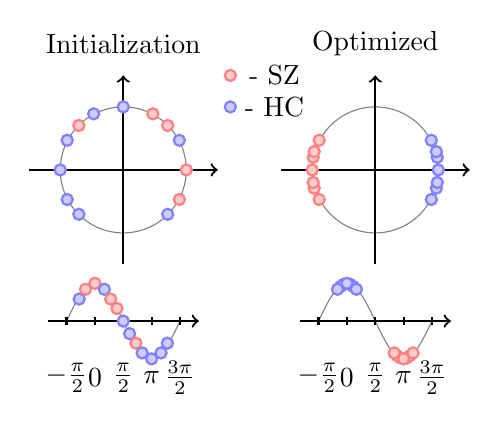
\begin{tikzpicture}
        [scale=0.8,
        inner sep=0.5mm,
        pd/.style={circle,draw=red!50,fill=red!20,thick},
        hc/.style={circle,draw=blue!50,fill=blue!20,thick}]
        
        %draw unit circle
        \node (uni_circle1) at (0,0) {};
        \draw[black!50, thin] ($(uni_circle1)$) circle [radius=1];
        \draw[black, thick, ->] ($(uni_circle1)+(-1.5,0)$) -- ($(uni_circle1)+(1.5,0)$);%xaxis
        \draw[black, thick, ->] ($(uni_circle1)+(0,-1.5)$) -- ($(uni_circle1)+(0,1.5)$);%yaxis
        
        \node (ind1) at ($(uni_circle1)+(1,0)$) [pd] {};
        \node (ind2) at ($(uni_circle1)+(0,1)$) [hc] {};
        \node (ind1) at ($(uni_circle1)+(-0.705,0.705)$) [pd] {};
        \node (ind1) at ($(uni_circle1)+(0.705,0.705)$) [pd] {};
        \node (ind1) at ($(uni_circle1)+(0.47,0.89)$) [pd] {};
        \node (ind2) at ($(uni_circle1)+(-1,0)$) [hc] {};
        \node (ind2) at ($(uni_circle1)+(-0.89,-0.47)$) [hc] {};
        \node (ind2) at ($(uni_circle1)+(-0.705,-0.705)$) [hc] {};
        \node (ind2) at ($(uni_circle1)+(0.89,0.47)$) [hc] {};
        \node (ind2) at ($(uni_circle1)+(-0.89,0.47)$) [hc] {};
        \node (ind2) at ($(uni_circle1)+(-0.47,0.89)$) [hc] {};
        \node (ind2) at ($(uni_circle1)+(0.89,-0.47)$) [pd] {};
        \node (ind2) at ($(uni_circle1)+(0.705,-0.705)$) [hc] {};
        
        
        \node (legend) at ($(uni_circle1)+(1.7,1)$) {};
        \node at ($(legend)+(0.7,0.5)$) {- SZ};
        \node at ($(legend)+(0.7,0)$) {- HC};
        \node at ($(legend)+(0,0.5)$) [pd] {};
        \node at ($(legend)+(0,0)$) [hc] {};
        
        %draw unit circle
        \node (uni_circle2) at ($(uni_circle1)+(4,0)$) {};
        \draw[black!50, thin] ($(uni_circle2)$) circle [radius=1];
        \draw[black, thick, ->] ($(uni_circle2)+(-1.5,0)$) -- ($(uni_circle2)+(1.5,0)$);%xaxis
        \draw[black, thick, ->] ($(uni_circle2)+(0,-1.5)$) -- ($(uni_circle2)+(0,1.5)$);%yaxis
        
        
        %individuals
        \node (ind1) at ($(uni_circle2)+(-1,0)$) [pd] {};
        \node (ind1) at ($(uni_circle2)+(-0.89,0.47)$) [pd] {};
        \node (ind1) at ($(uni_circle2)+(-0.985,0.2)$) [pd] {};
        \node (ind1) at ($(uni_circle2)+(-0.97,0.29)$) [pd] {};
        \node (ind1) at ($(uni_circle2)+(-0.89,-0.47)$) [pd] {};
        \node (ind1) at ($(uni_circle2)+(-0.97,-0.29)$) [pd] {};
        \node (ind1) at ($(uni_circle2)+(-0.985,-0.2)$) [pd] {};
        
        \node (ind2) at ($(uni_circle2)+(1,0)$) [hc] {};
        \node (ind1) at ($(uni_circle2)+(0.89,0.47)$) [hc] {};
        \node (ind1) at ($(uni_circle2)+(0.985,0.2)$) [hc] {};
        \node (ind1) at ($(uni_circle2)+(0.97,0.29)$) [hc] {};
        \node (ind1) at ($(uni_circle2)+(0.89,-0.47)$) [hc] {};
        \node (ind1) at ($(uni_circle2)+(0.97,-0.29)$) [hc] {};
        \node (ind1) at ($(uni_circle2)+(0.985,-0.2)$) [hc] {};
        
        
        
        \node (sinusoid1) at ($(uni_circle1)+(0,-2.7)$) {};
        \draw[black, thick, ->] ($(sinusoid1)+(-1.2,0.3)$) -- ($(sinusoid1)+(1.2,0.3)$);%xaxis
        \draw[thin, black!50] ($(sinusoid1)+(0.9,0.3)$) sin ($(sinusoid1)+(0.45,-0.3)$);
        \draw[thin, black!50] ($(sinusoid1)+(0.45,-0.3)$) cos ($(sinusoid1)+(0.,0.3)$);
        \draw[thin, black!50] ($(sinusoid1)+(0.,0.3)$) sin ($(sinusoid1)+(-0.45,0.9)$);
        \draw[thin, black!50] ($(sinusoid1)+(-0.45,0.9)$) cos ($(sinusoid1)+(-0.9,0.3)$);
        
        \draw[black, thick] ($(sinusoid1)+(-0.9,0.36)$) -- ($(sinusoid1)+(-0.9,0.24)$);
        
        \draw[black, thick] ($(sinusoid1)+(-0.45,0.36)$) -- ($(sinusoid1)+(-0.45,0.24)$);
        \draw[black, thick] ($(sinusoid1)+(0.,0.36)$) -- ($(sinusoid1)+(0.,0.24)$);
        \draw[black, thick] ($(sinusoid1)+(0.45,0.36)$) -- ($(sinusoid1)+(0.45,0.24)$);
        \draw[black, thick] ($(sinusoid1)+(0.9,0.36)$) -- ($(sinusoid1)+(0.9,0.24)$);
        
        \node at ($(sinusoid1)+(-0.9,-0.6)$) {$-\frac{\pi}{2}$};
        \node at ($(sinusoid1)+(-0.45,-0.6)$) {$0$};
        \node at ($(sinusoid1)+(0.,-0.6)$) {$\frac{\pi}{2}$};
        \node at ($(sinusoid1)+(0.45,-0.6)$) {$\pi$};
        \node at ($(sinusoid1)+(0.9,-0.6)$) {$\frac{3\pi}{2}$};
        
        \node (ind1) at ($(sinusoid1)+(-0.7,0.65)$) [hc] {};
        \node (ind1) at ($(sinusoid1)+(-0.6,0.805)$) [pd] {};
        \node (ind1) at ($(sinusoid1)+(-0.45,0.9)$) [pd] {};
        \node (ind1) at ($(sinusoid1)+(-0.3,0.805)$) [hc] {};
        \node (ind1) at ($(sinusoid1)+(-0.2,0.65)$) [pd] {};
        \node (ind1) at ($(sinusoid1)+(-0.1,0.5)$) [pd] {};
        \node (ind1) at ($(sinusoid1)+(0.,0.3)$) [hc] {};
        \node (ind1) at ($(sinusoid1)+(0.1,0.1)$) [hc] {};
        \node (ind1) at ($(sinusoid1)+(0.2,-0.05)$) [pd] {};
        \node (ind1) at ($(sinusoid1)+(0.3,-0.205)$) [hc] {};
        \node (ind1) at ($(sinusoid1)+(0.45,-0.3)$) [hc] {};
        \node (ind1) at ($(sinusoid1)+(0.6,-0.205)$) [hc] {};
        \node (ind1) at ($(sinusoid1)+(0.7,-0.05)$) [hc] {};
        
        \node (sinusoid2) at ($(uni_circle2)+(0,-2.7)$) {};
        \draw[black, thick, ->] ($(sinusoid2)+(-1.2,0.3)$) -- ($(sinusoid2)+(1.2,0.3)$);%xaxis
        \draw[thin, black!50] ($(sinusoid2)+(0.9,0.3)$) sin ($(sinusoid2)+(0.45,-0.3)$);
        \draw[thin, black!50] ($(sinusoid2)+(0.45,-0.3)$) cos ($(sinusoid2)+(0.,0.3)$);
        \draw[thin, black!50] ($(sinusoid2)+(0.,0.3)$) sin ($(sinusoid2)+(-0.45,0.9)$);
        \draw[thin, black!50] ($(sinusoid2)+(-0.45,0.9)$) cos ($(sinusoid2)+(-0.9,0.3)$);
        
        \draw[black, thick] ($(sinusoid2)+(-0.9,0.36)$) -- ($(sinusoid2)+(-0.9,0.24)$);
        
        \draw[black, thick] ($(sinusoid2)+(-0.45,0.36)$) -- ($(sinusoid2)+(-0.45,0.24)$);
        \draw[black, thick] ($(sinusoid2)+(0.,0.36)$) -- ($(sinusoid2)+(0.,0.24)$);
        \draw[black, thick] ($(sinusoid2)+(0.45,0.36)$) -- ($(sinusoid2)+(0.45,0.24)$);
        \draw[black, thick] ($(sinusoid2)+(0.9,0.36)$) -- ($(sinusoid2)+(0.9,0.24)$);
        
        \node at ($(sinusoid2)+(-0.9,-0.6)$) {$-\frac{\pi}{2}$};
        \node at ($(sinusoid2)+(-0.45,-0.6)$) {$0$};
        \node at ($(sinusoid2)+(0.,-0.6)$) {$\frac{\pi}{2}$};
        \node at ($(sinusoid2)+(0.45,-0.6)$) {$\pi$};
        \node at ($(sinusoid2)+(0.9,-0.6)$) {$\frac{3\pi}{2}$};
        
        
        \node (ind1) at ($(sinusoid2)+(-0.5,0.885)$) [hc] {};
        \node (ind1) at ($(sinusoid2)+(-0.55,0.85)$) [hc] {};
        \node (ind1) at ($(sinusoid2)+(-0.6,0.805)$) [hc] {};
        \node (ind1) at ($(sinusoid2)+(-0.4,0.885)$) [hc] {};
        \node (ind1) at ($(sinusoid2)+(-0.35,0.85)$) [hc] {};
        \node (ind1) at ($(sinusoid2)+(-0.3,0.805)$) [hc] {};
        \node (ind1) at ($(sinusoid2)+(-0.45,0.9)$) [hc] {};
        
        
        \node (ind1) at ($(sinusoid2)+(0.5,-0.285)$) [pd] {};
        \node (ind1) at ($(sinusoid2)+(0.55,-0.25)$) [pd] {};
        \node (ind1) at ($(sinusoid2)+(0.6,-0.205)$) [pd] {};
        \node (ind1) at ($(sinusoid2)+(0.4,-0.285)$) [pd] {};
        \node (ind1) at ($(sinusoid2)+(0.35,-0.25)$) [pd] {};
        \node (ind1) at ($(sinusoid2)+(0.3,-0.205)$) [pd] {};
        \node (ind1) at ($(sinusoid2)+(0.45,-0.3)$) [pd] {};
        
        \node (title1) at ($(uni_circle1)+(0,2)$) {Initialization};
        \node (title2) at ($(uni_circle2)+(0,2)$) {Optimized};
        
        %\node (stats1) at ($(uni_circle1)+(0,-4)$) {$\mathbb{E}[f_x(x)]=\frac{\pi}{2}, \mbox{Var}[f_x(x)]=\frac{\pi}{2}$};
        %\node (stats2) at ($(uni_circle2)+(0,-4)$) {$\mathbb{E}[f_x(x)]=\frac{\pi}{2}, \mbox{Var}[f_x(x)]=\frac{\pi}{2}$};
        
    \end{tikzpicture}
    \caption{Normalization of data points inside the unit circle, using layer normalization, along with the optimization of a contrastive loss lead to correct separation of sinusoids. Data points belong to two classes, $HC$ and $SZ$, that are separated after the minimization of $\mathcal{L}_D$. Because we separate false pairs, according to $(1-y_p) \times ||D(x_1,x_2)-m||_1$, all points are placed within a shift variant interval of the cosine. The variance needed for classification.}
    \label{fig:sinusoid_separation}
\end{figure}

\subsection{Dataset Characteristics}\label{materials:data}

Table~\ref{tab:data_description} summarises the datasets. All are previously published, anonymised public releases analysed here as secondary data.

\noindent\textbf{First-episode psychosis (FEP1, FEP2).} Two independently collected samples from the University of Pittsburgh (OpenNeuro ds003944 and ds003947) \cite{salisbury_ds003944,salisbury_ds003947}: individuals with a first episode of psychosis and healthy controls; five minutes of eyes-open resting EEG recorded with a 10-10 cap inside an Elekta Neuromag Vectorview MEG system (61 EEG channels, 1000\,Hz, reference TP9). Age, sex, symptom and functioning scales (BPRS, SANS, SAPS, GAF, SFS), cognition (MATRICS, WASI) and chlorpromazine-equivalent medication are released. FEP1 lists 82 recordings, but five people appear twice under the identifiers \texttt{sub-X} and \texttt{sub-XA} (same age, sex and race, recorded days apart); we kept one recording per person (47 patients, 30 controls). FEP2 contains 31 patients and 30 controls and excludes, by construction, the subjects shared with FEP1.

\noindent\textbf{Chronic schizophrenia (Semmelweis).} Resting EEG from Semmelweis University, Budapest \cite{racz2025}: 38 patients with schizophrenia and 39 age- and sex-matched controls; about two minutes of eyes-closed rest, 64-channel Neuroscan amplifier at 1000\,Hz. Patients are identified by the presence of PANSS ratings, which reproduces the 38/39 split of the source publication (35 of the 38 carry an ICD-10 F20/F25 code in the released table; three have a missing or non-F2 code). Medication, illness duration, education and PANSS scores are released.

\noindent\textbf{Parkinson's disease (PD).} Resting EEG from the University of New Mexico (OpenNeuro ds003490) \cite{cavanagh_ds003490}: 25 patients with Parkinson's disease and 25 matched controls; 63 EEG channels, 500\,Hz (Brain Vision ActiChamp, reference CPz), instructed one-minute eyes-closed and eyes-open spans, plus EOG and a three-axis accelerometer on the most tremor-affected hand. Patients were recorded twice, a week apart, ON and OFF dopaminergic medication (13 ON first, 12 OFF first); we analysed the OFF session. Eight subjects of this cohort were used by \cite{yao2025catd}.

\noindent\textbf{Schizophrenia spectrum, task EEG (Fribourg).} The cohort of the earlier version of this work \cite{dataset2022fribourg}: 19 patients with a psychotic disorder (ICD-10) and 24 controls, recorded during the Ultimatum Game (responder role), 128-channel Biosemi ActiveTwo at 2048\,Hz with additional EXG channels. The public release distributes the group label only; group-level characteristics are reported in \cite{horat2018impaired}.

\begin{table}[t]
    \centering
    \caption{Characteristics and roles of the datasets. \textit{pt}: patients; \textit{hc}: healthy controls; age as mean $\pm$ standard deviation (years); analysed EEG is the fixed crop used for every subject of a cohort.}
    \label{tab:data_description}
    \small
    \begin{tabular}{p{2.2cm} | p{2.5cm} | p{1.2cm} | p{2.3cm} | p{1.5cm} | p{4.2cm}}
        \hline
        \hline
         \hfil Dataset & \hfil Role / disease & \hfil pt/hc & \hfil Age pt | hc & \hfil Sex (M/F) pt | hc & \hfil Recording (analysed EEG) \\
         \hline
         NODDI & synthesis training & 0/16 & \hfil $32.8\pm8.1^{a}$ & \hfil 11/6$^{a}$ & rest, eyes open, simultaneous EEG-fMRI, 64 ch, 250\,Hz \\
         FEP1 (ds003944) & first-episode psychosis & 47/30 & $22.5\pm5.1$ | $21.6\pm4.1$ & 33/14 | 18/12 & rest, eyes open, 61 ch, 1\,kHz (300\,s) \\
         FEP2 (ds003947) & first-episode psychosis & 31/30 & $23.4\pm4.7$ | $24.2\pm5.1$ & 22/9 | 16/14 & rest, eyes open, 61 ch, 1\,kHz (300\,s) \\
         Semmelweis & schizophrenia (chronic) & 38/39 & $33.9\pm10.6$ | $32.7\pm9.7$ & 24/14 | 24/15 & rest, eyes closed, 64 ch, 1\,kHz (118\,s$^{b}$) \\
         PD (ds003490) & Parkinson's disease (OFF) & 25/25 & $69.7\pm8.7$ | $69.3\pm9.6$ & 16/9 | 16/9 & rest, eyes closed/open spans, 63 ch, 500\,Hz (400\,s) \\
         Fribourg (ds004000) & schizophrenia spectrum & 19/24 & n/a & n/a & Ultimatum Game, 128 ch, 2048\,Hz (400\,s) \\
         \hline
         \hline
    \end{tabular}

    \raggedright\footnotesize $^{a}$For the 17 acquired participants; version 2 of the release contains 16. $^{b}$One control recording is 109.7\,s long and was used in full.
\end{table}

\noindent\textbf{Leakage audit.} Before any modelling we tested, for every cohort, whether recording metadata predicts the diagnostic label (channel set, number of channels, sampling rate, filters, duration, recording date and hour, number of annotations, file size), checked for repeated participants and verified group sizes against the source publications.

\section{Experimental setting}\label{section:setting}\vskip0.2cm

The experiments compare, per cohort, the following views, each classified with an $l_2$-regularised logistic regression (Equation~\ref{equation:loss}): the \textit{bandpower} view $v_0$; the \textit{fmri} view $v_2$ of each synthesizer, reduced to 20 principal components; their combination $v_0 \oplus v_2$; the same \textit{fmri} and combined views from the untrained synthesizers; and the contrastive sinusoid-separation classifier of Section~\ref{methods:separation} (two variants). All transformations (standardisation, principal components) are fit on training folds only. All experiments were run on NVIDIA A100, H100 and L4 GPUs (synthesis) and CPU nodes (linear models).

\subsection{Validation}\label{section:validation}

To validate each view $v_i$, we perform repeated stratified 10-fold cross-validation at the subject level (20 repeats; 3 for the contrastive classifier), with one recording per person, and select the regularisation strength $C \in \{10^{-3},10^{-2},10^{-1},1,10\}$ by inner stratified 5-fold cross-validation within each training fold (Algorithm~\ref{alg:nested-cv}). We report the AUC averaged over repeats with a 95\% bootstrap confidence interval (2,000 stratified resamples of subjects), and a one-sided label-permutation $p$-value, $p=(1+\#\{\mathrm{AUC}_{\mathrm{perm}}\geq\mathrm{AUC}\})/(1+N)$, from $N=100$ permutations that each re-run the full nested procedure ($N=20$ for the contrastive classifier, minimum $p\approx0.048$). The added value of synthesis is $\Delta\mathrm{AUC}=\mathrm{AUC}(v_0\oplus v_2)-\mathrm{AUC}(v_0)$, with a paired bootstrap interval over subjects. Leave-one-subject-out estimates, used in the earlier version of this work, are reported only as a sensitivity analysis: with weak features they are biased below chance, because the class balance of each training set mirrors the held-out label \cite{varoquaux2018}.

\begin{algorithm}[t]
\caption{Nested repeated cross-validation for view $v_i$}
\label{alg:nested-cv}
\begin{algorithmic}[1]
\Require individuals $S$ with labels $y$; view $v_i$; hyperparameter grid $\mathcal{H}$; $R$ repeats
\Ensure AUC, out-of-fold probabilities $P$
\For{$r = 1$ \textbf{to} $R$}
    \For{each stratified fold $(S_{\text{train}}, S_{\text{test}})$ of $S$} \Comment{10 folds, subject level}
        \State fit standardisation (and PCA) on $S_{\text{train}}$ only
        \State $h^\star \gets \arg\max_{h \in \mathcal{H}} \textsc{CV}_5(v_i, S_{\text{train}}, h)$ \Comment{inner folds within $S_{\text{train}}$}
        \State fit $v_i$ with $h^\star$ on $S_{\text{train}}$; $P_r[S_{\text{test}}] \gets v_i.\textsc{predict}(S_{\text{test}})$
    \EndFor
\EndFor
\State \Return $\frac{1}{R}\sum_r \textsc{AUC}(P_r, y)$, $\frac{1}{R}\sum_r P_r$
\end{algorithmic}
\end{algorithm}

\subsection{Supporting synthesis analyses}\label{setting:fidelity}

The biclustering of the earlier version is not repeated: it was computed on synthesized volumes derived from leaked inputs (Section~\ref{section:res_leak}). Instead, to interpret the classification results we characterise what the synthesizers learn on NODDI. (a) \emph{Image protocol}: leave-one-subject-out over the 16 subjects (two validation subjects per fold for model selection), scored with SSIM, RMSE and voxelwise temporal correlation against an EEG-free population template (the mean training volume), with trigger-aligned EEG, EEG paired from the file start, and ECG only. (b) \emph{Fair target}: BOLD motion-corrected (rigid registration, FSL), cleaned with the Friston-24 motion model and spike regressors for framewise displacement above 0.5\,mm \cite{friston1996,power2014}, high-passed at 0.01\,Hz, z-scored, smoothed (6\,mm) and averaged into the 48 Harvard-Oxford grey-matter parcels present in every subject plus the global signal; ridge regression from lagged band power or full spectra, and UnEBOLT \cite{li2026unebolt} with its pretrained EEG encoder \cite{jiang2024labram}, predicted the parcel time series of held-out subjects. Significance used circular-shift and cross-subject swap nulls on detrended predictions and targets, and IAAFT surrogates of the BOLD with model refitting \cite{schreiber1996,mehta2025time}.

\section{Results}\label{section:results}

\subsection{Leakage audit}\label{section:res_leak}

In the Fribourg release, all 24 controls have 132 channels (128 EEG plus EXG1, EXG2, EXG7, EXG8), while 18 of the 19 patients have 134 (additionally EXG3, EXG4; Fisher $p=3\times10^{-11}$). The earlier pipeline kept the first 132 channels in file order, so its last two input channels were EXG7/EXG8 in controls and EXG3/EXG4 in patients. Reproducing its \textit{stft} features exactly and classifying them with a linear model under leave-one-subject-out validation gives a subject-level AUC of $0.965$; with 20\,s windows pooled across subjects, as in the earlier evaluation, AUC is $0.931$, matching the published $0.933$. With the 128 EEG channels only, AUC is $0.487$ (95\% CI $0.31$--$0.68$; permutation $p=0.46$); with the four auxiliary positions alone, $0.993$. Patients were also recorded in later years than controls (AUC $0.82$ for recording year). The earlier \textit{fmri} view ($0.765$) took the same 132-channel input and, at classification time, re-initialised the pretrained encoder, so it did not use the learned EEG-to-fMRI mapping. No metadata field predicted the label in FEP1 or PD; FEP2 recordings differed by 3\,s in median duration and Semmelweis patients were recorded earlier in the day (median 14\,h vs 16\,h), handled by fixed-length crops and noted as limitations.

\subsection{Classification}\label{section:res_clf}

Band power separated Parkinson's disease from controls (AUC $0.786$, 95\% CI $0.63$--$0.92$, $p=0.010$) but not the psychosis or schizophrenia cohorts (Table~\ref{tab:clf}): FEP1 $0.620$ ($p=0.12$), FEP2 $0.646$ ($p=0.06$), FEP1 and FEP2 pooled ($n=138$) $0.568$ ($p=0.14$), Semmelweis $0.571$ ($p=0.17$), Fribourg $0.539$ ($p=0.31$).

Synthesized fMRI did not exceed band power in any cohort. In Parkinson's disease, where band power discriminates, synthesized views also discriminated (E2fNet $0.741$, $p=0.01$; Spec2VolCAMU-Net $0.694$, $p=0.04$; NT-ViT $0.674$, $p=0.02$; CNN-TAG $0.484$, $p=0.54$). In the psychosis and schizophrenia cohorts, no synthesized view was significant except Spec2VolCAMU-Net in Semmelweis ($0.620$, $p=0.03$). Combining synthesized fMRI with band power changed AUC by $-0.046$ to $+0.112$; five of 20 intervals exclude or touch zero from above, none of which would survive a correction for 20 comparisons, and each is matched by its untrained control.

\noindent\textbf{Untrained synthesizers match trained ones.} Where synthesized views discriminated, the same architectures with random weights did as well or better: in Parkinson's disease $0.702$ (CNN-TAG), $0.707$ (E2fNet), $0.740$ (Spec2VolCAMU-Net) and $0.708$ (NT-ViT), against $0.484$, $0.741$, $0.694$ and $0.674$ trained; in Semmelweis the untrained Spec2VolCAMU-Net reached $0.738$ against $0.620$ trained, and its fusion gain ($+0.168$) exceeded the trained one ($+0.112$).

\noindent\textbf{Contrastive sinusoid separation.} The contrastive classifier discriminated only in Parkinson's disease, at the smallest attainable $p$, and stayed below band power there (Table~\ref{tab:contrastive}). Initialising the encoder from the NODDI-trained synthesizer did not improve on re-initialisation.

\begin{table*}[t]
    \centering
    \caption{AUC per cohort (repeated stratified 10-fold, mean over 20 repeats; permutation $p$ in parentheses). Trained / untrained: \textit{fmri} view of the synthesizer with learned or random weights. $\Delta$: AUC($v_0\oplus v_2$) $-$ AUC($v_0$) with 95\% paired bootstrap interval; uncorrected, 20 comparisons.}
    \label{tab:clf}
    \small
    \begin{tabular}{ p{1.8cm} | p{3.2cm} | p{1.8cm} | p{1.2cm} | p{3.0cm} | p{1.6cm}}
        \hline
        \hline
        \hfil Cohort & \hfil View & \hfil Trained & \hfil Untrained & \hfil $\Delta$ trained & \hfil $\Delta$ untrained\\
        \hline
        FEP1 & \textit{bandpower} & $0.620$ ($0.12$) & & & \\
         & CNN-TAG & $0.574$ ($0.21$) & $0.413$ & $-0.043$ [$-0.11$, $0.03$] & $-0.088$ \\
         & E2fNet & $0.527$ ($0.31$) & $0.634$ & $+0.005$ [$-0.08$, $0.08$] & $-0.008$ \\
         & Spec2VolCAMU-Net & $0.598$ ($0.12$) & $0.516$ & $-0.046$ [$-0.12$, $0.02$] & $+0.006$ \\
         & NT-ViT & $0.506$ ($0.34$) & $0.585$ & $-0.023$ [$-0.08$, $0.03$] & $+0.009$ \\
        \hline
        FEP2 & \textit{bandpower} & $0.646$ ($0.06$) & & & \\
         & CNN-TAG & $0.328$ ($1.00$) & $0.555$ & $-0.025$ [$-0.07$, $0.02$] & $+0.028$ \\
         & E2fNet & $0.572$ ($0.22$) & $0.571$ & $+0.000$ [$-0.04$, $0.04$] & $-0.001$ \\
         & Spec2VolCAMU-Net & $0.608$ ($0.16$) & $0.575$ & $+0.024$ [$-0.02$, $0.07$] & $-0.001$ \\
         & NT-ViT & $0.595$ ($0.06$) & $0.617$ & $+0.003$ [$-0.03$, $0.03$] & $-0.003$ \\
        \hline
        Semmelweis & \textit{bandpower} & $0.571$ ($0.17$) & & & \\
         & CNN-TAG & $0.583$ ($0.17$) & $0.562$ & $+0.010$ [$-0.05$, $0.07$] & $+0.071$ \\
         & E2fNet & $0.539$ ($0.29$) & $0.469$ & $+0.065$ [$0.01$, $0.12$] & $+0.004$ \\
         & Spec2VolCAMU-Net & $0.620$ ($0.03$) & $0.738$ & $+0.112$ [$0.04$, $0.20$] & $+0.168$ \\
         & NT-ViT & $0.471$ ($0.60$) & $0.587$ & $-0.018$ [$-0.11$, $0.08$] & $+0.094$ \\
        \hline
        PD & \textit{bandpower} & $\mathbf{0.786}$ ($0.01$) & & & \\
         & CNN-TAG & $0.484$ ($0.54$) & $0.702$ & $+0.019$ [$-0.00$, $0.05$] & $+0.018$ \\
         & E2fNet & $0.741$ ($0.01$) & $0.707$ & $+0.003$ [$-0.02$, $0.03$] & $+0.032$ \\
         & Spec2VolCAMU-Net & $0.694$ ($0.04$) & $0.740$ & $+0.035$ [$0.01$, $0.07$] & $-0.024$ \\
         & NT-ViT & $0.674$ ($0.02$) & $0.708$ & $+0.034$ [$0.01$, $0.07$] & $+0.022$ \\
        \hline
        Fribourg & \textit{bandpower} & $0.539$ ($0.31$) & & & \\
         & CNN-TAG & $0.597$ ($0.15$) & $0.555$ & $+0.000$ [$-0.07$, $0.06$] & $+0.004$ \\
         & E2fNet & $0.532$ ($0.31$) & $0.554$ & $+0.075$ [$0.00$, $0.15$] & $+0.061$ \\
         & Spec2VolCAMU-Net & $0.608$ ($0.11$) & $0.498$ & $+0.009$ [$-0.05$, $0.06$] & $+0.044$ \\
         & NT-ViT & $0.614$ ($0.12$) & $0.565$ & $+0.007$ [$-0.03$, $0.04$] & $+0.031$ \\
        \hline
        \hline
    \end{tabular}
\end{table*}

\begin{table}[t]
    \centering
    \caption{Contrastive sinusoid separation: AUC (repeated stratified 10-fold, 3 repeats), 95\% bootstrap interval and permutation $p$ (20 permutations; minimum $0.048$).}
    \label{tab:contrastive}
    \small
    \begin{tabular}{ p{1.6cm} | p{3.3cm} | p{3.3cm} | p{1.4cm}}
        \hline
        \hline
        \hfil Cohort & \hfil As in 2023 & \hfil Pretrained encoder & \hfil \textit{bandpower} \\
        \hline
        FEP1 & $0.485$ [$0.39$, $0.67$] ($0.57$) & $0.599$ [$0.48$, $0.73$] ($0.19$) & $0.620$ \\
        FEP2 & $0.476$ [$0.34$, $0.63$] ($0.52$) & $0.433$ [$0.27$, $0.54$] ($0.76$) & $0.646$ \\
        Semmelweis & $0.538$ [$0.46$, $0.72$] ($0.33$) & $0.562$ [$0.45$, $0.70$] ($0.24$) & $0.571$ \\
        PD & $0.701$ [$0.58$, $0.86$] ($0.048$) & $0.660$ [$0.53$, $0.82$] ($0.048$) & $0.786$ \\
        Fribourg & $0.559$ [$0.38$, $0.74$] ($0.33$) & $0.602$ [$0.44$, $0.77$] ($0.14$) & $0.539$ \\
        \hline
        \hline
    \end{tabular}
\end{table}

\subsection{What the synthesizers learn}\label{section:res_fidelity}

On NODDI, the EEG-free template reaches SSIM $0.676$ and PSNR $21.2$ under the protocol of \cite{roos2025brainwaves}, at or above the published values of E2fNet ($0.605$), NT-ViT ($0.581$) and Spec2VolCAMU-Net ($0.693$), and above the $0.46$ of the earlier version of this synthesizer \cite{calhas2022eeg}. Retrained with trigger-aligned EEG, all synthesizers lost to or tied the template (SSIM $0.631$--$0.669$ against $0.675$; RMSE worse, $p\leq0.02$), performed the same with EEG paired from the file start or with ECG alone, and showed no voxelwise temporal correlation beyond shifted or swapped EEG after detrending, motion regression and selection of steady-state volumes (three seeds; edge and interior voxels). With the fair target, EEG predicted a statistically detectable but negligible part of BOLD in held-out subjects: ridge from full spectra $r=0.026$, UnEBOLT $r=0.035$ (above shift and swap nulls, $p=0.02$ and $p=0.03$), with $R^2\approx0$ for both; within subjects, $r\approx0$.

\section{Discussion}\label{section:discussion}

\noindent\textbf{Synthesized fMRI does not improve EEG-based diagnosis in these cohorts.} With four synthesizers, a contrastive fine-tuning method and five cohorts, no synthesized view outperformed EEG band power, and its addition to band power produced no gain beyond that of untrained networks of the same architecture. Where synthesized fMRI discriminated patients from controls, most clearly in Parkinson's disease, the discriminative content was what these networks extract from EEG spectra regardless of training. Fine-tuning the synthesizer's sinusoid space with the contrastive loss did not change this, and starting it from the learned mapping gave no advantage over starting from random weights.

\noindent\textbf{Why.} A synthesized volume can only carry information present in the EEG it is computed from, and the supporting analyses show how little of that information is haemodynamic. Under the image protocol used by published synthesizers, models reproduce the static anatomy that an EEG-free template already captures and ignore EEG timing; under a fair BOLD target, EEG predicts a statistically detectable but negligible share of the variance, even with a state-of-the-art model. The psychosis and schizophrenia cohorts add a second limit: resting band power itself discriminated only weakly there, so there was little EEG signal for any view to transform.

\noindent\textbf{How a positive result arose.} The earlier version of this work reported AUC $0.93$ for the \textit{stft} view and $0.77$ for the synthesized \textit{fmri} view in the Fribourg cohort, and spatial patterns in frontal, temporal and cerebellar regions. Those results are explained by the auxiliary-channel layout of the public release, which encodes the diagnosis when channels are selected by position, and the synthesized view did not use the learned mapping. Two further protocol issues of the NODDI benchmark, EEG-fMRI misalignment from the file start and positional channel indexing across two montages, are shared by several pipelines and are invisible to SSIM and PSNR, which an EEG-free template already maximises. We recommend that synthesis studies report an EEG-free template and temporal metrics against shift and swap nulls, and that diagnostic uses of synthesized fMRI report an EEG-only baseline, untrained-network controls and a leakage audit of the clinical data.

\section{Related work}\label{section:related_work}

\noindent\textbf{EEG-to-fMRI synthesis.} Convolutional transcoders \cite{liu2019convolutional, liu2020latent}, attention- and Fourier-feature-based encoder-decoders \cite{calhas2022eeg}, U-Net and Mamba decoders \cite{roos2025brainwaves,he2025spec2vol}, vision transformers \cite{lanzino2024ntvit} and diffusion models \cite{yao2025catd} synthesize volumes, while NeuroBOLT and UnEBOLT \cite{li2024neurobolt,li2026unebolt} and distributed-lag models \cite{mehta2025time} predict region time series; the latter work showed, within subjects and with surrogate tests, that EEG predicts BOLD in task-relevant regions. Downstream diagnostic use has been reported for schizophrenia \cite{calhas2023medrxiv} and Parkinson's disease \cite{yao2025catd}.

\noindent\textbf{Schizophrenia.}\label{related_work:schizophrenia} Schizophrenia is marked by cognitive and structural brain alterations \cite{sui2018multimodal}. fMRI-based classification of controls and patients has shown promise \cite{de2019machine}, with consistent findings of frontal and temporal volume reductions \cite{chin2018recognition} and white-matter abnormalities \cite{cetin2020white}. EEG-based classification is common, but its pitfalls, including small samples and validation that is not at the subject level, have been documented \cite{barros2021advanced}; our leakage audit adds dataset-level shortcuts to that list.

\noindent\textbf{Interpretability.}\label{related_work:interpretability} For EEG, interpretability remains a challenge. \citet{pinto2022interpretable} applied evolutionary feature selection and \textit{apriori} association rules to explain seizure detection, identifying key features across spectral, temporal, and electrode dimensions. Band power, used here as the EEG baseline, is itself spatially organised over the scalp and has established clinical interpretations in schizophrenia \cite{roach2008event,bates2009low}; the case for synthesized fMRI as a more interpretable view would require spatial maps validated against real fMRI in patients, which the present data cannot provide.

\section{Conclusion}\label{section:conclusion}

In five public cohorts spanning first-episode psychosis, chronic schizophrenia and Parkinson's disease, EEG-synthesized fMRI did not improve classification over EEG band power, its discriminative content was reproduced by untrained networks, and the contrastive sinusoid-separation method did not change this. Claims that synthesized fMRI aids diagnosis should be tested against EEG-only baselines, untrained-network controls and leakage audits. The contrastive formulation itself extends to more than two classes, as sketched below, but its value depends on the synthesized space carrying diagnostic information beyond the EEG, which we did not find. A multi class solution is to consider the unitary circle in Figure \ref{future_work:fig:multi_label_sinusoid}. Let the pairs of data be $(x_1, x_2, y_1, y_2, y_p)$. By definition $x_1 := \mathbf{x}_2 \in \mathbb{R}^E$. And consider the targets $y_1, y_2 \in [0,1]^C$. Now $y_p$ instead of being in $[0,1]$, consider $y_p=||argmax(y_1) - argmax(y_2)||_1^1 \times \frac{\pi}{C}$ so that the possible values are $\in \{0,\frac{\pi}{C}, \dots, \frac{C\pi}{C}\}$. The contrastive loss now only needs one of its terms and can be written as
\begin{equation}\label{future_work:equation:multi_contrastive}
    \mathcal{L}_D(x_1, x_2, y_p) = ||D(x_1, x_2)-y_p||_1^1 .
\end{equation}
The other change that is needed is to apply the softmax at the output of the classifier, so that $y\in \Delta^C$.

\begin{figure}[ht]
    \centering
    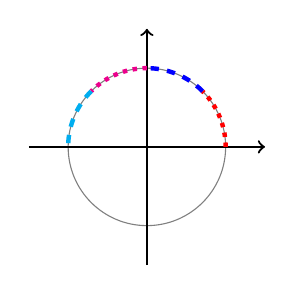
\begin{tikzpicture}
        [scale=1.,
        inner sep=0.5mm,
        pd/.style={circle,draw=red!50,fill=red!20,thick},
        hc/.style={circle,draw=blue!50,fill=blue!20,thick}]
        
        %draw unit circle
        \node (uni_circle1) at (0,0) {};
        \draw[black!50, thin] ($(uni_circle1)$) circle [radius=1];
        \draw[black, thick, ->] ($(uni_circle1)+(-1.5,0)$) -- ($(uni_circle1)+(1.5,0)$);%xaxis
        \draw[black, thick, ->] ($(uni_circle1)+(0,-1.5)$) -- ($(uni_circle1)+(0,1.5)$);%yaxis       

        \draw [dotted, ultra thick,red,domain=0:45] plot ({cos(\x)}, {sin(\x)});
        \draw [dashed, ultra thick,blue,domain=45:90] plot ({cos(\x)}, {sin(\x)});
        \draw [dotted, ultra thick,magenta,domain=90:135] plot ({cos(\x)}, {sin(\x)});
        \draw [dashed, ultra thick,cyan,domain=135:180] plot ({cos(\x)}, {sin(\x)});

        
    \end{tikzpicture}
    \caption{Hypothesis to separate multiple groups of data using the sinusoid projection. The example considers $C=4$.}
    \label{future_work:fig:multi_label_sinusoid}
\end{figure}

\section*{Limitations}

Sample sizes are modest (43--77 subjects per cohort), so AUC intervals are wide; null results bound but do not exclude small effects. Resting EEG carried weak signal in the psychosis and schizophrenia cohorts, so the evaluation is most informative in Parkinson's disease. The synthesizers were trained on one resting-state, eyes-open, 1.5\,T dataset of 16 healthy adults; the clinical EEG differed in system, montage (interpolated), eye condition (Semmelweis eyes closed) and paradigm (Fribourg task), and no clinical cohort has paired fMRI, so synthesis fidelity in patients cannot be measured. Patients were medicated in the psychosis and schizophrenia cohorts, and Semmelweis patients were recorded earlier in the day. Each subject's synthesized sequence was summarised by its temporal mean and standard deviation; other summaries, such as synthesized connectivity, were not tested. The contrastive classifier used fixed hyperparameters and fewer permutations than the other views. CATD could not be evaluated, and NeuroBOLT/UnEBOLT were used for fidelity only.

\section*{Social impact}

Synthesized neuroimaging using EEG has been presented as a scalable, low-cost alternative for mental health diagnostics. Our results caution against deploying it for diagnosis before it is shown to add information beyond the EEG itself, and show that public clinical datasets can contain shortcuts that make such methods appear accurate. While this study used publicly available, consented datasets, real-world use demands rigorous clinical validation and secure data governance. Environmental impact is also a concern; thus, energy-efficient, low-resource AI methods are encouraged.


\subsection*{Ethics statement}

All procedures performed in this study involving human participants were in accordance with the ethical standards of the institutional and/or national research committee and with the 1964 Helsinki Declaration and its later amendments or comparable ethical standards. The research was conducted in compliance with relevant laws and institutional guidelines.

This study involved the secondary analysis of anonymized public data:
\begin{itemize}
    \item NODDI Dataset: Collected by \citet{dataset_01} with ethics commmittee approval ID ID:4290/001;
    \item First-episode psychosis datasets (OpenNeuro ds003944, ds003947): University of Pittsburgh \verify{approval ID};
    \item Semmelweis dataset: Semmelweis University \cite{racz2025} \verify{approval ID};
    \item Parkinson's disease dataset (OpenNeuro ds003490): University of New Mexico \verify{approval ID};
    \item Fribourg Dataset: Collected by \citet{dataset2022fribourg} with ethics commmittee approval ID 054/13-CER-FR.
\end{itemize}

\bibliographystyle{unsrtnat}
%\bibliography{references}
\begin{thebibliography}{57}
\providecommand{\natexlab}[1]{#1}
\providecommand{\url}[1]{\texttt{#1}}
\expandafter\ifx\csname urlstyle\endcsname\relax
  \providecommand{\doi}[1]{doi: #1}\else
  \providecommand{\doi}{doi: \begingroup \urlstyle{rm}\Url}\fi

\bibitem[Saha et~al.(2005)]{saha2005systematic}
Sukanta Saha et~al.
\newblock A systematic review of the prevalence of schizophrenia.
\newblock \emph{PLoS medicine}, 2005.

\bibitem[Andreou et~al.(2020)]{andreou2020structural}
Christina Andreou et~al.
\newblock Structural and functional imaging markers for susceptibility to psychosis.
\newblock \emph{Molecular psychiatry}, 2020.

\bibitem[Neale et~al.(2015)]{neale2015genetic}
Benjamin~M Neale et~al.
\newblock Genetic analysis of schizophrenia and bipolar disorder reveals polygenicity but also suggests new directions for molecular interrogation.
\newblock \emph{Current opinion in neurobiology}, 2015.

\bibitem[Corcoran et~al.(2020)]{corcoran2020language}
Cheryl~M Corcoran et~al.
\newblock Language as a biomarker for psychosis: {A} natural language processing approach.
\newblock \emph{Schizophrenia research}, 2020.

\bibitem[TAN et~al.(2016)]{tan2016eeg}
O{\u{g}}uz TAN et~al.
\newblock Eeg complexity and frequency in chronic residual schizophrenia.
\newblock \emph{Anatolian Journal of Psychiatry/Anadolu Psikiyatri Dergisi}, 2016.

\bibitem[Ayd{\i}n et~al.(2018)]{aydin2018cortical}
Serap Ayd{\i}n et~al.
\newblock Cortical correlations in wavelet domain for estimation of emotional dysfunctions.
\newblock \emph{Neural Computing and Applications}, 2018.

\bibitem[Oh et~al.(2020)]{oh2020identifying}
Jihoon Oh et~al.
\newblock Identifying schizophrenia using structural {MRI} with a deep learning algorithm.
\newblock \emph{Frontiers in psychiatry}, 2020.

\bibitem[Velakoulis et~al.(2006)]{velakoulis2006hippocampal}
Dennis Velakoulis et~al.
\newblock Hippocampal and amygdala volumes according to psychosis stage and diagnosis: {A} magnetic resonance imaging study of chronic schizophrenia, first-episode psychosis, and ultra--high-risk individuals.
\newblock \emph{Archives of general psychiatry}, 2006.

\bibitem[Haukvik et~al.(2013)]{haukvik2013schizophrenia}
Unn~Kristin Haukvik et~al.
\newblock Schizophrenia--what does structural {MRI} show?
\newblock \emph{Tidsskrift for Den norske legeforening}, 2013.

\bibitem[Ogbole et~al.(2018)]{ogbole2018survey}
Godwin~Inalegwu Ogbole et~al.
\newblock Survey of magnetic resonance imaging availability in {W}est {A}frica.
\newblock \emph{Pan African Medical Journal}, 2018.

\bibitem[Liu et~al.(2019)]{liu2019convolutional}
Xueqing Liu et~al.
\newblock A convolutional neural network for transcoding simultaneously acquired {EEG}-f{MRI} data.
\newblock In \emph{NER}, 2019.

\bibitem[Liu et~al.(2020)]{liu2020latent}
Xueqing Liu et~al.
\newblock Latent neural source recovery via transcoding of simultaneous {EEG}-f{MRI}.
\newblock \emph{arXiv}, 2020.

\bibitem[Bricman et~al.(2021)]{bricman2021eeg2fmri}
Paul Bricman et~al.
\newblock {EEG}2f{MRI}: {C}ross-{M}odal {S}ynthesis for {F}unctional {N}euroimaging.
\newblock \emph{Github}, 2021.

\bibitem[Calhas et~al.(2023)]{calhas2022eeg}
David Calhas et~al.
\newblock Eeg to fmri synthesis benefits from attentional graphs of electrode relationships.
\newblock \emph{MLHC}, 2023.

\bibitem[Mehta et~al.(2025)]{mehta2025time}
Neil Mehta et~al.
\newblock Time-varying {EEG} spectral power predicts evoked and spontaneous f{MRI} motor brain activity.
\newblock \emph{arXiv}, 2025.

\bibitem[Li et~al.(2024)]{li2024neurobolt}
Yamin Li et~al.
\newblock Neurobolt: Resting-state {EEG}-to-f{MRI} synthesis with multi-dimensional feature mapping.
\newblock \emph{Advances in Neural Information Processing Systems}, 2024.

\bibitem[Roos et~al.(2025)]{roos2025brainwaves}
Kristofer~Grover Roos et~al.
\newblock From {B}rainwaves to {B}rain {S}cans: {A} {R}obust {N}eural {N}etwork for {EEG}-to-f{MRI} {S}ynthesis.
\newblock \emph{arXiv}, 2025.

\bibitem[Treviso et~al.(2020)]{treviso2020explanation}
Marcos~V Treviso et~al.
\newblock The explanation game: {T}owards prediction explainability through sparse communication.
\newblock \emph{arXiv}, 2020.

\bibitem[Barros et~al.(2021)]{barros2021advanced}
Carla Barros et~al.
\newblock Advanced eeg-based learning approaches to predict schizophrenia: Promises and pitfalls.
\newblock \emph{Artificial intelligence in medicine}, 114:\penalty0 102039, 2021.

\bibitem[Fingelkurts et~al.(2007)]{fingelkurts2007impaired}
Andrew~A Fingelkurts et~al.
\newblock Impaired functional connectivity at {EEG} alpha and theta frequency bands in major depression.
\newblock \emph{Human brain mapping}, 2007.

\bibitem[Burgess et~al.(2002)]{burgess2002functional}
Adrian~P Burgess et~al.
\newblock Functional connectivity of gamma {EEG} activity is modulated at low frequency during conscious recollection.
\newblock \emph{International {J}ournal of {{P}}sychophysiology}, 2002.

\bibitem[Albrecht et~al.(2018)]{albrecht2018time}
Matthew~A Albrecht et~al.
\newblock Time and frequency dependent changes in resting state {EEG} functional connectivity following lipopolysaccharide challenge in rats.
\newblock \emph{PLoS One}, 2018.

\bibitem[Roach et~al.(2008)]{roach2008event}
Brian~J Roach et~al.
\newblock Event-related {EEG} time-frequency analysis: {A}n overview of measures and an analysis of early gamma band phase locking in schizophrenia.
\newblock \emph{Schizophrenia bulletin}, 2008.

\bibitem[Bates et~al.(2009)]{bates2009low}
Alan~T Bates et~al.
\newblock Low-frequency {EEG} oscillations associated with information processing in schizophrenia.
\newblock \emph{Schizophrenia research}, 2009.

\bibitem[Jacobsen et~al.(2003)]{jacobsen2003sliding}
Eric Jacobsen et~al.
\newblock The sliding {DFT}.
\newblock \emph{{IEEE} Signal Processing Magazine}, 2003.

\bibitem[He et~al.(2016)]{he2016deep}
Kaiming He et~al.
\newblock Deep residual learning for image recognition.
\newblock In \emph{CVPR}, 2016.

\bibitem[Rahimi et~al.(2007)]{rahimi2007random}
Ali Rahimi et~al.
\newblock Random {F}eatures for {L}arge-{S}cale {K}ernel {M}achines.
\newblock In \emph{NIPS}, 2007.

\bibitem[Tancik et~al.(2020)]{tancik2020fourier}
Matthew Tancik et~al.
\newblock Fourier features let networks learn high frequency functions in low dimensional domains.
\newblock \emph{arXiv}, 2020.

\bibitem[Padée et~al.(2022)]{dataset2022fribourg}
Anna Padée et~al.
\newblock "fribourg {U}ltimatum {G}ame in {S}chizophrenia {S}tudy", 2022.

\bibitem[Deligianni et~al.(2014)]{dataset_01}
Fani Deligianni et~al.
\newblock Relating resting-state f{MRI} and {EEG} whole-brain connectomes across frequency bands.
\newblock \emph{Frontiers in Neuroscience}, 2014.

\bibitem[Ba et~al.(2016)]{ba2016layer}
Jimmy~Lei Ba et~al.
\newblock Layer normalization.
\newblock \emph{ar{X}iv}, 2016.

\bibitem[Horat et~al.(2018)]{horat2018impaired}
Sibylle~K Horat et~al.
\newblock Impaired social cognition in schizophrenia during the ultimatum game: An eeg study.
\newblock \emph{Schizophrenia research}, 2018.

\bibitem[Itil(1977)]{itil1977qualitative}
Turan~M Itil.
\newblock Qualitative and quantitative eeg findings in schizophrenia.
\newblock \emph{Schizophrenia bulletin}, 1977.

\bibitem[Sui et~al.(2018)]{sui2018multimodal}
Jing Sui et~al.
\newblock Multimodal neuromarkers in schizophrenia via cognition-guided {MRI} fusion.
\newblock \emph{Nature communications}, 2018.

\bibitem[de~Filippis et~al.(2019)]{de2019machine}
Renato de~Filippis et~al.
\newblock Machine learning techniques in a structural and functional {MRI} diagnostic approach in schizophrenia: {A} systematic review.
\newblock \emph{Neuropsychiatric disease and treatment}, 2019.

\bibitem[Chin et~al.(2018)]{chin2018recognition}
Rowena Chin et~al.
\newblock Recognition of schizophrenia with regularized support vector machine and sequential region of interest selection using structural magnetic resonance imaging.
\newblock \emph{Scientific Reports}, 2018.

\bibitem[Cetin-Karayumak et~al.(2020)]{cetin2020white}
Suheyla Cetin-Karayumak et~al.
\newblock White matter abnormalities across the lifespan of schizophrenia: a harmonized multi-site diffusion {MRI} study.
\newblock \emph{Molecular psychiatry}, 2020.

\bibitem[Pinto et~al.(2022)]{pinto2022interpretable}
Mauro Pinto et~al.
\newblock Interpretable {EEG} seizure prediction using a multiobjective evolutionary algorithm.
\newblock \emph{Scientific reports}, 2022.


\bibitem[Calhas et~al.(2023b)]{calhas2023medrxiv}
David Calhas et~al.
\newblock {EEG} to {fMRI} synthesis to aid medical decision: {A} schizophrenia case study \verify{title and authors}.
\newblock \emph{medRxiv}, 10.1101/2023.08.07.23293748, 2023.

\bibitem[Yao et~al.(2025)]{yao2025catd}
Weiheng Yao et~al.
\newblock {CATD}: Unified representation learning for {EEG}-to-{fMRI} cross-modal generation.
\newblock \emph{IEEE Transactions on Medical Imaging}, 2025.

\bibitem[He et~al.(2025)]{he2025spec2vol}
Dongyi He et~al.
\newblock {Spec2VolCAMU-Net}: A spectrogram-to-volume model for {EEG}-to-{fMRI} reconstruction \verify{title and authors}.
\newblock \emph{Journal of Neural Engineering}, 2025.

\bibitem[Lanzino et~al.(2024)]{lanzino2024ntvit}
Romeo Lanzino et~al.
\newblock {NT-ViT}: Neural transcoding vision transformers for {EEG}-to-{fMRI} synthesis.
\newblock In \emph{ECCV Workshops}, 2024.

\bibitem[Li et~al.(2026)]{li2026unebolt}
Yamin Li et~al.
\newblock {UnEBOLT}: A unified model for {EEG}-to-{BOLD} translation and functional connectivity reconstruction \verify{venue}.
\newblock In \emph{Medical Imaging with Deep Learning (MIDL)}, 2026.

\bibitem[Deligianni et~al.(2016)]{deligianni2016}
Fani Deligianni et~al.
\newblock {NODDI} and tensor-based microstructural indices as predictors of functional connectivity.
\newblock \emph{PLoS ONE}, 2016.

\bibitem[Salisbury et~al.(2021a)]{salisbury_ds003944}
Dean F. Salisbury et~al.
\newblock {EEG}: First episode psychosis vs. control resting task 1 \verify{authors}.
\newblock OpenNeuro ds003944, 2021.

\bibitem[Salisbury et~al.(2021b)]{salisbury_ds003947}
Dean F. Salisbury et~al.
\newblock {EEG}: First episode psychosis vs. control resting task 2 \verify{authors}.
\newblock OpenNeuro ds003947, 2021.

\bibitem[Racz et~al.(2025)]{racz2025}
Frigyes Samuel Racz et~al.
\newblock Reduced temporal variability of cortical excitation/inhibition ratio in schizophrenia.
\newblock \emph{Schizophrenia}, 11:\penalty0 20, 2025.

\bibitem[Cavanagh(2021)]{cavanagh_ds003490}
James F. Cavanagh.
\newblock {EEG}: 3-stim auditory oddball and rest in {Parkinson's} \verify{title}.
\newblock OpenNeuro ds003490, 2021.

\bibitem[Varoquaux(2018)]{varoquaux2018}
Ga{\"e}l Varoquaux.
\newblock Cross-validation failure: Small sample sizes lead to large error bars.
\newblock \emph{NeuroImage}, 180:\penalty0 68--77, 2018.

\bibitem[Friston et~al.(1996)]{friston1996}
Karl J. Friston et~al.
\newblock Movement-related effects in {fMRI} time-series.
\newblock \emph{Magnetic Resonance in Medicine}, 35\penalty0 (3):\penalty0 346--355, 1996.

\bibitem[Power et~al.(2014)]{power2014}
Jonathan D. Power et~al.
\newblock Methods to detect, characterize, and remove motion artifact in resting state {fMRI}.
\newblock \emph{NeuroImage}, 84:\penalty0 320--341, 2014.

\bibitem[Schreiber and Schmitz(1996)]{schreiber1996}
Thomas Schreiber and Andreas Schmitz.
\newblock Improved surrogate data for nonlinearity tests.
\newblock \emph{Physical Review Letters}, 77\penalty0 (4):\penalty0 635, 1996.

\bibitem[Jiang et~al.(2024)]{jiang2024labram}
Wei-Bang Jiang et~al.
\newblock Large brain model for learning generic representations with tremendous {EEG} data in {BCI}.
\newblock In \emph{ICLR}, 2024.

\end{thebibliography}

\normalsize


\clearpage
\newpage
\appendix

\begin{proof}
Let $\phi(z) = \left[ \cos(\omega_1^\top z + \beta_1), \dots, \cos(\omega_d^\top z + \beta_d) \right]$, where each $\omega_i \sim \mathcal{N}(0, I_d)$ and $\beta_i \sim \mathrm{Uniform}[0, 2\pi]$. The inner product between projected vectors is:
\[
\phi(z_1)^\top \phi(z_2) = \sum_{i=1}^d \cos(\omega_i^\top z_1 + \beta_i) \cos(\omega_i^\top z_2 + \beta_i).
\]
Using the trigonometric identity:
\[
\cos(a)\cos(b) = \frac{1}{2}[\cos(a - b) + \cos(a + b)],
\]
we write:
\begin{align*}
    &\cos(\omega_i^\top z_1 + \beta_i) \cos(\omega_i^\top z_2 + \beta_i) = \\
&\frac{1}{2} \left[ \cos(\omega_i^\top(z_1 - z_2)) + \cos(\omega_i^\top(z_1 + z_2) + 2\beta_i) \right].    
\end{align*}


Taking the expectation over $\beta_i \sim \mathrm{Uniform}[0, 2\pi]$, the second term vanishes:
\[
\mathbb{E}_{\beta_i}[\cos(\omega_i^\top(z_1 + z_2) + 2\beta_i)] = 0.
\]

Thus,
\[
\mathbb{E}_{\omega, \beta}[\phi(z_1)^\top \phi(z_2)] = \frac{1}{2} \sum_{i=1}^d \mathbb{E}_{\omega_i}[\cos(\omega_i^\top(z_1 - z_2))].
\]

Let $\delta = z_1 - z_2$. Since $\omega_i^\top \delta \sim \mathcal{N}(0, \|\delta\|_2^2)$, we use the identity:
\[
\mathbb{E}_{x \sim \mathcal{N}(0, \sigma^2)}[\cos(x)] = e^{-\frac{1}{2}\sigma^2},
\]
to obtain:
\[
\mathbb{E}_{\omega_i}[\cos(\omega_i^\top \delta)] = e^{-\frac{1}{2}\|\delta\|_2^2}.
\]

Putting it together:
\[
\mathbb{E}_{\omega, \beta}[\phi(z_1)^\top \phi(z_2)] = \frac{d}{2} e^{-\frac{1}{2}\|z_1 - z_2\|_2^2}.
\]

Therefore, for any $\|z_1 - z_2\|_2 > 0$, we have:
\[
\mathbb{E}_{\omega, \beta}[\phi(z_1)^\top \phi(z_2)] < \frac{d}{2} < d,
\]
proving the result.
\end{proof}

\clearpage
\newpage

\end{document}